\twocolumn[\colorsection{Segundo principio de la termodinámica}]
\setcounter{figure}{0}
%
\begin{Exercise}
  En un calorímetro ideal (adiabático y de capacidad calorífica despreciable) se introducen $\SI{50}{\gram}$ de agua a $\SI{15}{\celsius}$ y $\SI{50}{\gram}$ de agua a $\SI{5}{\celsius}$, y se espera hasta que el sistema (la mezcla) alcance el equilibrio térmico. \textit{a}) Calcule la variación de entropía del sistema. \textit{b}) ¿Cuál es la variación de entropía del Universo en este proceso?
\end{Exercise}
\begin{Answer}
	\begin{minipage}[t]{.4\textwidth}
    \textit{a}) $\SI{0.016}{cal/\kelvin}$\\ \textit{b}) $\SI{0.016}{cal/\kelvin}$
  \end{minipage}
\end{Answer}
%
\begin{Exercise}
  Un bloque de hielo de $\SI{4.5}{\kilogram}$ a $\SI{0}{\celsius}$ cae en el océano y se funde. La temperatura media del océano es $\SI{3.5}{\celsius}$, incluyendo las aguas profundas. ¿En qué medida la fusión de este hielo cambia la entropía del mundo? ¿La aumenta o la disminuye? (La variación de la temperatura del océano mientras este bloque de hielo se funde es despreciable.)
\end{Exercise}
\begin{Answer}
	\begin{minipage}[t]{.4\textwidth}
    $\Delta S = \SI{71.3}{\joule/\kelvin}$
  \end{minipage}
\end{Answer}
%
\begin{Exercise}
  Un motor diesel realiza $\SI{2200}{\joule}$ de trabajo mecánico y cede $\SI{4300}{\joule}$ de calor en cada ciclo. \textit{a}) ¿Cuánto calor debe suministrarse al motor en cada ciclo? \textit{b}) Calcule la eficiencia térmica del motor.
\end{Exercise}
\begin{Answer}
	\begin{minipage}[t]{.4\textwidth}
    \textit{a}) $\SI{6500}{\joule}$\\ \textit{b}) 34\%
  \end{minipage}
\end{Answer}
%
\begin{Exercise}\label{p:segundoppio01}
  \ifthenelse{\equal{\seleccionados}{true}}
  {\addToList{xyz-segundoppio}{\ExerciseHeaderNB}}{}
  La figura \ref{f:segundoppio01} muestra un esquema de una máquina térmica cuyo depósito de alta temperatura está a una temperatura $T_c = \SI{620}{\kelvin}$, recibe $Q_\text{abs} = \SI{550}{\joule}$ de calor a esta temperatura en cada ciclo y cede $Q_\text{ced} = \SI{-395}{\joule}$ al depósito frío, a una temperatura $T_f = \SI{378}{\kelvin}$. \textit{a}) ¿Cuánto trabajo mecánico realiza la máquina en cada ciclo? \textit{b}) ¿Cuál es la eficiencia térmica de la máquina? \textit{c}) ¿Se trata de una máquina ideal o real?
\end{Exercise}
\begin{Answer}
	\begin{minipage}[t]{.4\textwidth}
    \textit{a}) $W = \SI{155}{\joule}$\\ \textit{b}) $e = 0.282$\\ \textit{c}) la máquina es real
  \end{minipage}
\end{Answer}
%
\begin{center}
  \begin{tikzpicture}[scale=1]
      
    % It needs:
    % \documentclass[dvipsnames]{article}
    % \usepackage{xcolor}
    % \usetikzlibrary{arrows.meta}
    
    \draw [rounded corners, thick, fill=pink] (0,4) rectangle (3,5);
    \draw [rounded corners, thick, fill=cyan] (0,0) rectangle (3,1);
    \draw [thick, fill=LimeGreen] (1.5,2.5) circle [radius=0.5];
    \draw (1.5,4.5) node {$T_c$};
    \draw (1.5,0.5) node {$T_f$};
    \draw (1.5,2.5) node {gas};

    \draw [color=pink] [-{Triangle[width=25pt,length=8pt]}, line width=18pt](1.5,3.95) -- (1.5, 3);
    \draw (1.5,3.5) node {$Q_c$};
    \draw [color=cyan] [-{Triangle[width=25pt,length=8pt]}, line width=18pt](1.5,1.97) -- (1.5, 1);
    \draw (1.5,1.5) node {$Q_f$};
    \draw [color=LimeGreen] [-{Triangle[width=25pt,length=8pt]}, line width=18pt](2.02,2.5) -- (3.5, 2.5);
    \draw (2.75,2.5) node {$W$};

  \end{tikzpicture}
  \captionof{figure}{Problema \ref{p:segundoppio01}\label{f:segundoppio01}}
\end{center}
%
\begin{Exercise}\label{p:segundoppio02}
  En la tabla \ref{t:segundoppio02} se muestra el calor absorbido, el calor cedido (en valor absoluto) y el trabajo realizado en cada ciclo de cuatro máquinas térmicas diseñadas para funcionar entre dos reservorios a temperaturas constantes de $\SI{800}{\kelvin}$ y $\SI{400}{\kelvin}$. ¿Cuáles de estas máquinas son posibles, debido a que no violan ningún principio termodinámico?\\
  \begin{table}[h]
    \caption{Ejercicio \ref{p:segundoppio02}}\label{t:segundoppio02}
    \centering
    \begin{tabular}{cccc}
        \hline
        \textbf{Máquina} & \textbf{$Q$ abs. [J]} & \textbf{$Q$ ced. [J]} & \textbf{$W$ [J]}\\
        \hline
        \textit{a} & 1000 & 600 & 600\\
        \textit{b} & 1000 & 400 & 600\\
        \textit{c} & 1000 & 500 & 500\\
        \textit{d} & 1000 & 700 & 300\\
        \hline
    \end{tabular}
  \end{table}
\end{Exercise}
\begin{Answer}
	\begin{minipage}[t]{.4\textwidth}
    Máquinas \textit{c} y \textit{d}
  \end{minipage}
\end{Answer}
%
\begin{Exercise}
  Un refrigerador tiene un coeficiente de rendimiento de $2.10$. Durante cada ciclo, absorbe $\SI{3.4E4}{\joule}$ de calor del depósito frío. \textit{a}) ¿Cuánta energía mecánica se requiere en cada ciclo para operar el refrigerador? \textit{b}) Durante cada ciclo, ¿cuánto calor se desecha al depósito caliente?
\end{Exercise}
\begin{Answer}
	\begin{minipage}[t]{.4\textwidth}
    \textit{a}) $\SI{1.62E4}{\joule}$\\ \textit{b}) $\SI{5.02E4}{\joule}$
  \end{minipage}
\end{Answer}
%
\begin{Exercise}
  Un acondicionador de aire tiene un coeficiente de rendimiento de $2.9$ en un día caluroso, y utiliza $\SI{850}{\watt}$ de potencia eléctrica. \textit{a}) ¿Cuántos Joules de calor extrae el sistema de aire acondicionado de la habitación en cada minuto? \textit{b}) ¿Cuántos Joules de calor entrega el sistema de aire acondicionado al aire caliente del exterior en cada minuto?
\end{Exercise}
\begin{Answer}
	\begin{minipage}[t]{.4\textwidth}
    \textit{a}) $\SI{148}{\kilo\joule}$\\ \textit{b}) $\SI{199}{\kilo\joule}$
  \end{minipage}
\end{Answer}
%
\begin{Exercise}
  \ifthenelse{\equal{\seleccionados}{true}}
  {\addToList{xyz-segundoppio}{\ExerciseHeaderNB}}{}
  Una máquina de Carnot opera entre $\SI{500}{\celsius}$ y $\SI{100}{\celsius}$ con un suministro de calor de $\SI{250}{\joule}$ por ciclo. \textit{a}) ¿Cuánto calor se entrega al depósito frío en cada ciclo? \textit{b}) ¿Qué número mínimo de ciclos se requieren para que la máquina levante una piedra de $\SI{500}{\kilogram}$ a una altura de $\SI{100}{\metre}$?
\end{Exercise}
\begin{Answer}
	\begin{minipage}[t]{.4\textwidth}
    \textit{a}) $\SI{121}{\joule}$\\ \textit{b}) $\SI{3.79E3}{ciclos}$
  \end{minipage}
\end{Answer}
%
\begin{Exercise}
  Una máquina de Carnot tiene una eficiencia del 59\% y realiza $\SI{25}{\kilo\joule}$ de trabajo en cada ciclo. \textit{a}) ¿Cuánto calor extrae la máquina de su fuente de calor en cada ciclo? \textit{b}) Suponga que la máquina expulsa calor a una temperatura ambiente de $\SI{20}{\celsius}$. ¿Cuál es la temperatura de su fuente de calor?
\end{Exercise}
\begin{Answer}
  \begin{minipage}[t]{.4\textwidth}
    \textit{a}) $\SI{42.37}{\kilo\joule}$; \textit{b}) $\SI{442}{\celsius}$
  \end{minipage}
\end{Answer}
%
\begin{Exercise}\label{p:segundoppio05}
  Calcule la eficiencia térmica de una máquina en la que $n$ moles de un gas ideal diatómico realizan el ciclo $1 \rightarrow 2 \rightarrow 3 \rightarrow 4 \rightarrow 1$ que se muestra en la figura \ref{f:segundoppio05}.
\end{Exercise}
\begin{Answer}
  \begin{minipage}[t]{.4\textwidth}
    $e = 2/19$
  \end{minipage}
\end{Answer}
%
\begin{center}
  \begin{tikzpicture}[scale=0.9]
    \begin{axis}[
      % ticks=none,
      axis x line=bottom,
      axis y line=left,
      xmin=0.5, xmax=2.5,
      ymin=0.5, ymax=2.5, 
      xlabel={$V$},
      ylabel={$p$},
      xtick={1,2},
      xticklabels={$V_0$,$2V_0$},
      ytick={1,2},
      yticklabels={$p_0$,$2p_0$}
      ];
    \addplot[color = black, dashed, thick] coordinates {(0, 2) (1, 2)};
    \addplot[color = black, dashed, thick] coordinates {(0, 1) (1, 1)};
    \addplot[color = black, dashed, thick] coordinates {(1, 0) (1, 1)};
    \addplot[color = black, dashed, thick] coordinates {(2, 0) (2, 1)};
    \draw [color=blue, very thick][-latex](1,2)--(1.5,2);
    \draw [color=blue, very thick](1.5,2)--(2,2);
    \draw [color=blue, very thick][-latex](2,2)--(2,1.5);
    \draw [color=blue, very thick](2,1.5)--(2,1);
    \draw [color=blue, very thick][-latex](2,1)--(1.5,1);
    \draw [color=blue, very thick](1.5,1)--(1,1);
    \draw [color=blue, very thick][-latex](1,1)--(1,1.5);
    \draw [color=blue, very thick](1,1.5)--(1,2);
    \draw (1,1) node [below left] {1};
    \draw (1,2) node [above left] {2};
    \draw (2,2) node [above right] {3};
    \draw (2,1) node [below right] {4};
    \fill [black](1,1) circle(2pt);
    \fill [black](1,2) circle(2pt);
    \fill [black](2,2) circle(2pt);
    \fill [black](2,1) circle(2pt);
    \end{axis}
  \end{tikzpicture}
  \captionof{figure}{Problema \ref{p:segundoppio05}\label{f:segundoppio05}}
\end{center}
%
\begin{Exercise}\label{p:segundoppio06}
  Calcule la eficiencia térmica de una máquina en la que $n$ moles de un gas ideal diatómico realizan el ciclo mostrado en la figura \ref{f:segundoppio06}.
\end{Exercise}
\begin{Answer}
	\begin{minipage}[t]{.4\textwidth}
    $e = \ln{(3)}/(2\ln{(3)}+7/2)$
  \end{minipage}
\end{Answer}
%
\begin{center}
  \begin{tikzpicture}[scale=0.9]
    \begin{axis}[
      % ticks=none,
      axis x line=bottom,
      axis y line=left,
      xmin=0.5, xmax=2.5,
      ymin=0.5, ymax=3.5, 
      xlabel={$T$},
      ylabel={$p$},
      xtick={1,2},
      xticklabels={$T_0$,$2T_0$},
      ytick={1,3},
      yticklabels={$p_0$,$3p_0$}
      %extra x ticks={0.04},
      %extra y ticks={2}
      ];
    \addplot[color = black, dashed, thick] coordinates {(0, 3) (1, 3)};
    \addplot[color = black, dashed, thick] coordinates {(0, 1) (1, 1)};
    \addplot[color = black, dashed, thick] coordinates {(1, 0) (1, 1)};
    \addplot[color = black, dashed, thick] coordinates {(2, 0) (2, 1)};
    % \addplot[color = black, dashed, thick] coordinates {(9, 0) (9, 1.5)};
    \draw [color=blue, very thick][-latex](1,3)--(1.5,3);
    \draw [color=blue, very thick](1.5,3)--(2,3);
    \draw [color=blue, very thick][-latex](2,3)--(2,2);
    \draw [color=blue, very thick](2,2)--(2,1);
    \draw [color=blue, very thick][-latex](2,1)--(1.5,1);
    \draw [color=blue, very thick](1.5,1)--(1,1);
    \draw [color=blue, very thick][-latex](1,1)--(1,2);
    \draw [color=blue, very thick](1,2)--(1,3);
    \fill [black](1,1) circle(2pt);
    \fill [black](1,3) circle(2pt);
    \fill [black](2,3) circle(2pt);
    \fill [black](2,1) circle(2pt);
    \end{axis}
  \end{tikzpicture}
  \captionof{figure}{Problema \ref{p:segundoppio06}\label{f:segundoppio06}}
\end{center}
%
\begin{Exercise}
  Un cilindro contiene oxígeno a una presión de $\SI{2.00}{atm}$, en un volumen de $\SI{4.00}{\liter}$ y a una temperatura de $\SI{300}{\kelvin}$. Suponga que el oxígeno se puede tratar como gas ideal mientras se somete a los siguientes procesos: \textit{i}) Calentamiento a presión constante desde el estado inicial (estado 1) al estado 2, donde $T = \SI{450}{\kelvin}$. \textit{ii}) Enfriamiento a volumen constante hasta $\SI{250}{\kelvin}$ (estado 3). \textit{iii}) Compresión a temperatura constante hasta un volumen de $\SI{4.00}{\liter}$ (estado 4). \textit{iv}) Calentamiento a volumen constante hasta $\SI{300}{\kelvin}$, regresando el sistema al estado 1. Determine la eficiencia de este dispositivo como máquina térmica y compárela con la de una máquina de ciclo de Carnot que opera entre las mismas temperaturas mínima y máxima de $\SI{250}{\kelvin}$ y $\SI{450}{\kelvin}$.
\end{Exercise}
\begin{Answer}
	\begin{minipage}[t]{.4\textwidth}
    $7.5\%$ (el máximo posible es $44.4\%$)
  \end{minipage}
\end{Answer}
%
\begin{Exercise}\label{p:segundoppio04}
  Una máquina térmica opera siguiendo aproximadamente el ciclo de la figura \ref{f:segundoppio04}. Dos moles de helio gaseoso, que puede ser considerado como gas ideal, son utilizados como la sustancia de trabajo en esta máquina, que alcanza una temperatura máxima de $\SI{327}{\celsius}$ cuando llega al equilibrio con la fuente de temperatura alta. El proceso $bc$ es isotérmico reversible manteniendo al gas en contacto con la fuente de temperatura, la presión en los estados $a$ y $c$ es $\SI{100}{\kilo\pascal}$, y en el estado $b$ es $\SI{300}{\kilo\pascal}$. La temperatura de la fuente fría es la misma que alcanza el gas cuando llega al estado \textit{a}. \textit{a}) ¿Cuánto calor entra en el gas y cuánto sale del gas en cada ciclo? \textit{b}) ¿Cuánto trabajo efectúa la máquina en cada ciclo? \textit{c}) ¿Qué eficiencia tiene esta máquina? \textit{d}) Calcule el porcentaje que representa la eficiencia de esta máquina respecto de la máxima eficiencia posible que puede lograrse con los depósitos caliente y frío que se usan en este ciclo ($e_\text{máquina}/e_\text{máximo}\times 100\%$). \textit{e}) Si se invierte el sentido del ciclo para transformarla en una máquina refrigeradora, ¿la máquina que se obtiene es posible? (Verificar que se cumplan ambos principios de la termodinámica.)
\end{Exercise}
\begin{Answer}
	\begin{minipage}[t]{.4\textwidth}
    \textit{a}) Entran $\SI{20.9}{\kilo\joule}$ y salen $\SI{16.6}{\kilo\joule}$\\ \textit{b}) $\SI{4.3}{\kilo\joule}$\\ \textit{c}) 21\%\\ \textit{d}) La eficiencia de esta máquina es 31\% del máximo posible.
  \end{minipage}
\end{Answer}
%
\begin{center}
  \begin{tikzpicture}[scale=0.9]
    \begin{axis}[
      ticks=none,
      axis x line=bottom,
      axis y line=left,
      xmin=0.01, xmax=0.12,
      ymin=50, ymax=350, 
      xlabel={$V$},
      ylabel={$p$},
      ];
    \addplot [color=blue, very thick] [samples= 180, domain=0.033:0.066]  {100};
    \addplot [latex-, color=blue, very thick] [samples= 180, domain=0.066:0.1]  {100};
    \addplot [-latex, color=blue, very thick] [samples= 180, domain=0.033:0.066]  {100*0.1/x};
    \addplot [color=blue, very thick] [samples= 180, domain=0.066:0.1]  {100*0.1/x};
    \draw [color=blue, very thick][-latex](0.033,100)--(0.033,200);
    \draw [color=blue, very thick](0.033,200)--(0.033,300);
    \draw (0.033,100) node [left] {$a$};
    \draw (0.033,300) node [left] {$b$};
    \draw (0.1,100) node [above right] {$c$};
    \fill [black](0.033,100) circle(2pt);
    \fill [black](0.033,300) circle(2pt);
    \fill [black](0.1,100) circle(2pt);
    \end{axis}
  \end{tikzpicture}
  \captionof{figure}{Problema \ref{p:segundoppio04}\label{f:segundoppio04}}
\end{center}
%
\begin{Exercise}\label{p:segundoppio03}
  \ifthenelse{\equal{\seleccionados}{true}}
  {\addToList{xyz-segundoppio}{\ExerciseHeaderNB}}{}
  El diagrama $p$-$V$ de la figura \ref{f:segundoppio03} muestra un ciclo de una máquina térmica que usa $\SI{0.250}{\mole}$ de un gas ideal para el cual el coeficiente de dilatación adiabática es $\gamma = 1.40$. La parte curva $ab$ del ciclo corresponde a un proceso adiabático. \textit{a}) ¿Cuánto calor absorbe este gas por ciclo, y en qué parte del ciclo ocurre? \textit{b}) ¿Cuánto calor cede este gas por ciclo, y en qué parte del ciclo ocurre? \textit{c}) ¿Cuánto trabajo realiza esta máquina en un ciclo? \textit{d}) ¿Cuál es la eficiencia térmica de la máquina?
\end{Exercise}
\begin{Answer}
	\begin{minipage}[t]{.4\textwidth}
    \textit{a}) $\SI{5480}{\joule}$\\ \textit{b}) $\SI{3720}{\joule}$\\ \textit{c}) $\SI{1760}{\joule}$\\ \textit{d}) 32\%
  \end{minipage}
\end{Answer}
%
\begin{center}
  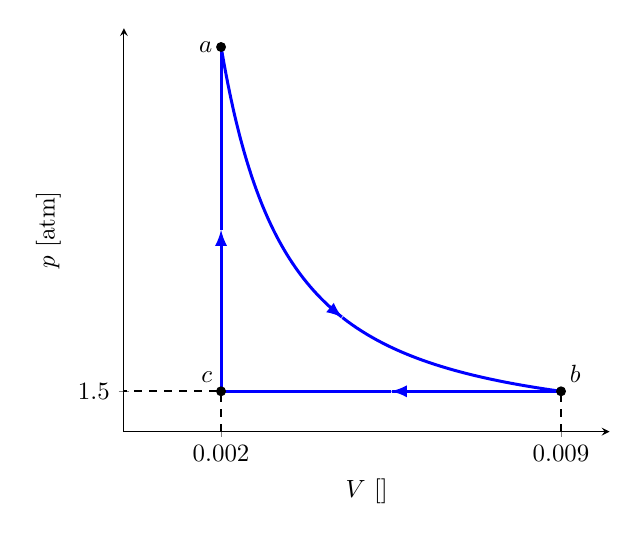
\begin{tikzpicture}[scale=0.9]
    \begin{axis}[
      %ticks=none,
      axis x line=bottom,
      axis y line=left,
      xmin=0, xmax=10,
      ymin=0, ymax=15, 
      xlabel={$V$~[$\si{\cubic\metre}$]},
      ylabel={$p$~[atm]},
      xtick={2,9},
      xticklabels={0.002,0.009},
      ytick={1.5},
      yticklabels={1.5}
      %yticklabels={},
      %extra x ticks={0.04},
      %extra y ticks={2}
      ];
    \addplot [color=blue, very thick] [samples= 180, domain=2:5.5]  {1.5};
    \addplot [latex-, color=blue, very thick] [samples= 180, domain=5.5:9]  {1.5};
    \addplot [-latex, color=blue, very thick] [samples= 180, domain=2:4.5]  {1.5*(9/x)^1.5};
    \addplot [color=blue, very thick] [samples= 180, domain=4.5:9]  {1.5*(9/x)^1.5};
    \addplot[color = black, dashed, thick] coordinates {(2, 0) (2, 1.5) (0, 1.5)};
    \addplot[color = black, dashed, thick] coordinates {(9, 0) (9, 1.5)};
    \draw [color=blue, very thick][-latex](2,1.5)--(2,7.5);
    \draw [color=blue, very thick](2,7.5)--(2,14.3);
    \draw (2,14.3) node [left] {$a$};
    \draw (9,1.5) node [above right] {$b$};
    \draw (2,1.5) node [above left] {$c$};
    \fill [black](2,14.3) circle(2pt);
    \fill [black](9,1.5) circle(2pt);
    \fill [black](2,1.5) circle(2pt);
    \end{axis}
  \end{tikzpicture}
  \captionof{figure}{Problema \ref{p:segundoppio03}\label{f:segundoppio03}}
\end{center}
%
\begin{Exercise}
  Una planta generadora de energía eléctrica de $\SI{1000}{\mega\watt}$, alimentada con carbón, tiene una eficiencia térmica del 40\%. \textit{a}) ¿Cuál es la rapidez de suministro de calor a la planta? \textit{b}) La planta quema carbón de piedra (antracita), que tiene un calor de combustión de $\SI{2.65E7}{\joule/\kilogram}$. ¿Cuánto carbón consume la planta al día, si opera de manera continua? \textit{c}) El depósito frío hacia donde la planta cede calor es un río cercano. La temperatura del río es $\SI{18.0}{\celsius}$ antes de llegar a la planta de energía y $\SI{18.5}{\celsius}$ después de recibir el calor de desecho de la planta. Calcule el caudal del río en $\si{\cubic\metre/\second}$.
\end{Exercise}
\begin{Answer}
	\begin{minipage}[t]{.4\textwidth}
    \textit{a}) $\SI{2500}{\mega\watt}$\\ \textit{b}) $\SI{8150}{ton}$\\ \textit{c}) $\SI{720}{\cubic\metre/\second}$
  \end{minipage}
\end{Answer}
%
\begin{Exercise}\label{p:segundoppio07}
  La figura \ref{f:segundoppio07} muestra el ciclo de Stirling idealizado, donde el proceso $1 \rightarrow 2$ es una expansión isotérmica a alta temperatura ($T_\text{c}$) y el proceso $3 \rightarrow 4$ es una compresión isotérmica a baja temperatura ($T_\text{f}$). \textit{a}) En un motor Stirling, las transferencias de calor en $4 \rightarrow 1$ y $2 \rightarrow 3$ no implican fuentes de calor externas, sino que usan regeneración: la misma sustancia que transfiere calor al gas del interior del cilindro en el proceso $4 \rightarrow 1$ absorbe calor del gas en el proceso $2 \rightarrow 3$. Por lo tanto, los calores transferidos $Q_{41}$ y $Q_{23}$ no afectan a la eficiencia del motor. Explique esta afirmación demostrando que se cumple $Q_{41} = - Q_{23}$. \textit{b}) Deduzca la eficiencia de este ciclo en términos de las temperaturas $T_\text{c}$ y $T_\text{f}$, teniendo en cuenta que representa a un motor Stirling que utiliza regeneración.
\end{Exercise}
\begin{Answer}
	\begin{minipage}[t]{.4\textwidth}
    \textit{b}) $e = 1 - T_f/T_c$
  \end{minipage}
\end{Answer}
%
\begin{center}
  \begin{tikzpicture}[scale=0.9]
    \begin{axis}[
      % ticks=none,
      axis x line=bottom,
      axis y line=left,
      xmin=0, xmax=5,
      ymin=0, ymax=450, 
      xlabel={$V$},
      ylabel={$p$},
      xtick={2,4},
      xticklabels={$V_1$,$V_2$},
      ytick=\empty,
      yticklabels={}
      %extra x ticks={0.04},
      %extra y ticks={2}
      ];
    \addplot [-latex, color=red, very thick] [samples= 180, domain=2:3] {600/x};
    \addplot [color=red, very thick] [samples= 180, domain=3:4] {600/x};
    \addplot [color=red, dashed, thick] [samples= 180, domain=1.4:2] {600/x};
    \addplot [color=red, dashed, thick] [samples= 180, domain=4:5] {600/x};
    \addplot [latex-, color=blue, very thick] [samples= 180, domain=3:4] {300/x};
    \addplot [color=blue, very thick] [samples= 180, domain=2:3] {300/x};
    \addplot [color=blue, dashed, thick] [samples= 180, domain=0.7:2] {300/x};
    \addplot [color=blue, dashed, thick] [samples= 180, domain=4:5] {300/x};
    
    \addplot[-latex, color = black, very thick] coordinates {(2, 150) (2, 225)};
    \addplot[color = black, very thick] coordinates {(2, 225) (2, 300)};
    \addplot[-latex, color = black, very thick] coordinates {(4, 150) (4, 112)};
    \addplot[color = black, very thick] coordinates {(4, 112) (4, 75)};

    \addplot[color = black, dashed, thick] coordinates {(2, 0) (2, 150)};
    \addplot[color = black, dashed, thick] coordinates {(4, 0) (4, 75)};
    
    \draw (2,150) node [below left] {4};
    \draw (2,300) node [below left] {1};
    \draw (4,150) node [above right] {2};
    \draw (4,75) node [below right] {3};
    \fill [black](2,150) circle(2pt);
    \fill [black](2,300) circle(2pt);
    \fill [black](4,150) circle(2pt);
    \fill [black](4,75) circle(2pt);
    \end{axis}
  \end{tikzpicture}
  \captionof{figure}{Problema \ref{p:segundoppio07}\label{f:segundoppio07}}
\end{center}
%
\begin{Exercise}\label{p:segundoppio08}
  El ciclo de la figura \ref{f:segundoppio08} aproxima el funcionamiento de una máquina térmica constituida por $\SI{0.55}{\mole}$ de un gas ideal diatómico que intercambia calor con dos depósitos que mantienen sus temperaturas constantes. El gas comienza en el estado $a$ con un volumen de $\SI{2.3}{\liter}$ y a la temperatura del reservorio caliente, $\SI{520}{\kelvin}$. Se expande adiabáticamente hasta un volumen de $\SI{9.0}{\liter}$, llegando al estado $b$ cuya temperatura es la del reservorio frío, $\SI{300}{\kelvin}$. Luego se comprime isotérmicamente hasta el estado $c$ con un volumen de $\SI{1.5}{\liter}$. Por último evoluciona sobre la trayectoria rectilínea que une los estados $c$ y $a$ para completar el ciclo. Calcular la eficiencia térmica de esta máquina. 
\end{Exercise}
\begin{Answer}
	\begin{minipage}[t]{.4\textwidth}
    $0.254$
  \end{minipage}
\end{Answer}
%
\begin{center}
  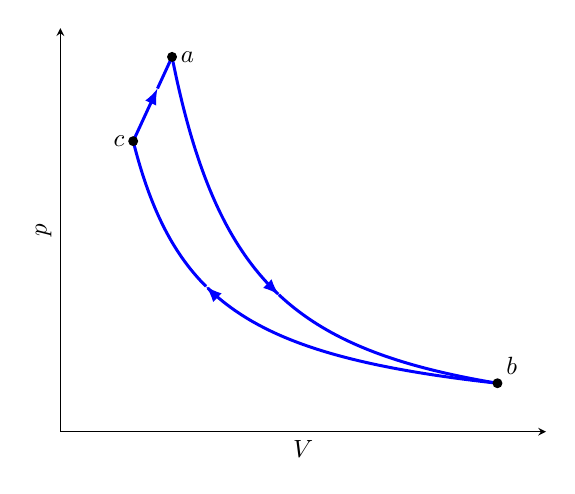
\begin{tikzpicture}[scale=0.9]
    \begin{axis}[
      ticks=none,
      axis x line=bottom,
      axis y line=left,
      xmin=0, xmax=10, 
      ymin=0, ymax=12.5, 
      xlabel={$V$},
      ylabel={$p$},
      % xtick={2,9},
      % xticklabels={1.5,9},
      % ytick={1.5},
      % yticklabels={1.5}
      %yticklabels={},
      %extra x ticks={0.04},
      %extra y ticks={2}
      ];
    \addplot [-latex, color=blue, very thick] [samples= 180, domain=2.3:4.5]  {1.5*(9/x)^1.5};
    \addplot [color=blue, very thick] [samples= 180, domain=4.5:9]  {1.5*(9/x)^1.5};
    \addplot [latex-, color=blue, very thick] [samples= 180, domain=3:9]  {1.5*9/x};
    \addplot [color=blue, very thick] [samples= 180, domain=1.5:3]  {1.5*9/x};
    % \addplot[color = black, dashed, thick] coordinates {(2, 0) (2, 1.5) (0, 1.5)};
    % \addplot[color = black, dashed, thick] coordinates {(9, 0) (9, 1.5)};
    \draw [color=blue, very thick][-latex](1.5,9)--(2,10.63);
    \draw [color=blue, very thick](2,10.63)--(2.3,11.61);
    \draw (2.3,11.61) node [right] {$a$};
    \draw (9,1.5) node [above right] {$b$};
    \draw (1.5,9) node [left] {$c$};
    \fill [black](2.3,11.61) circle(2pt);
    \fill [black](9,1.5) circle(2pt);
    \fill [black](1.5,9) circle(2pt);
    \end{axis}
  \end{tikzpicture}
  \captionof{figure}{Problema \ref{p:segundoppio08}\label{f:segundoppio08}}
\end{center}
%
